\documentclass[11pt,letterpaper]{article}
\usepackage{times}
\usepackage[onehalfspacing]{setspace}
\usepackage{natbib}\bibpunct{(}{)}{,}{}{}{,}
\usepackage{amsmath,amsfonts,amsthm}
\usepackage{comment}
\usepackage{tabularx}
\usepackage{multirow}
\usepackage{booktabs}
\usepackage{subcaption}
\usepackage{graphicx}
\usepackage[colorlinks,linkcolor=blue,citecolor=black,urlcolor=black]{hyperref}
\usepackage[title,titletoc]{appendix}
\usepackage{enumitem}
\usepackage{subcaption}  % For subfigures
\usepackage{lscape}      % For landscape orientation if needed
\usepackage[noabbrev,capitalize]{cleveref}
\usepackage{tikz}
\usetikzlibrary{shapes.geometric}
\usetikzlibrary{intersections} 
\usepackage{pgfplots}
\pgfplotsset{compat=1.18}
\usetikzlibrary{patterns, pgfplots.fillbetween}
\usepackage{graphicx}
\usepackage{mathpazo}

% commands
\newtheorem{definition}{Definition}
\newtheorem{proposition}{Proposition}
\newtheorem{lemma}{Lemma}
\newcommand{\figpath}{fig/}
\newcommand{\tablepath}{table/}
\newcommand{\rmdi}{\mathrm{d}}

% table and figure formatting
%\input{formats}

% page size
\setlength{\textwidth}{\paperwidth}
\addtolength{\textwidth}{-1.7in}
\setlength{\oddsidemargin}{.85in}
\addtolength{\oddsidemargin}{-.85in}
\setlength{\evensidemargin}{\oddsidemargin}
\setlength{\headheight}{0pt}
\setlength{\headsep}{0pt}
\setlength{\textheight}{\paperheight}
\addtolength{\textheight}{-\headheight}
\addtolength{\textheight}{-\headsep}
\addtolength{\textheight}{-\footskip}
\addtolength{\textheight}{-1.75in}
\setlength{\topmargin}{1in}
\addtolength{\topmargin}{-1in}

\begin{document}

\title{\textbf{Diverse Firms and Trade: the Melitz Model}}
\author{\large%
\setcounter{footnote}{0}%
Carlos G\'{o}es \\[-3pt] \textit{\small IFC, World Bank Group}
}
\maketitle

\paragraph{Preliminaries} Consider a world with two countries $i \in \{H,F \}$. The countries are identical in their populations $L_H=L_F$, preferences and production technologies. We will first describe these components of the economy and characterize the autarky equilibrium. We will then explore what happens if a country opens up to trade. 

\paragraph{Demand} Consumers in country $i$ supply their labor inelastically and earn labor income $w_i L_i$. They have preferences over many goods $\varphi \in \Phi_i$ where $\Phi_i$ is the set of all goods available in the domestic economy.

Economists use a constant elasticity-of-substitution (CES) utility function to capture preferences in a flexible way. The key parameter,  $\sigma > 1$ is the elasticity of substitution: the larger $\sigma$ is, the more readily consumers switch between varieties when their relative prices change (think “Coke vs. Pepsi” with a high $\sigma$). When $\sigma$ is close to 1, varieties are harder to substitute --each feels almost like a distinct necessity -- so consumers tolerate bigger price gaps before adjusting their baskets.

\begin{equation*}
    \max_{\{q_i(\
\varphi)\}_{\
\varphi \in \Phi_i}} Q_i \equiv \left[ \sum_{\varphi \in \Phi_i } q_i(
\varphi)^{\tfrac{\sigma-1}{\sigma}} \right]^{\tfrac{\sigma}{\sigma-1} } \qquad s.t. \qquad  P_i Q_i =\sum_{\varphi \in \Phi_i } p_i(\varphi) q_i(\varphi) \le I_i = w_i L_i + \Pi_i
\end{equation*}

First, a note on notation. $q_i(\varphi)$ and $p_i(\varphi)$ are the quantity demanded and price in country $i$ of the good $\varphi \in \Phi_i:=\{\varphi_{\min}, \varphi_{\min}+1, \varphi_{\min}+2, \cdots, \varphi_{\max}\}$. This is a small modification from what you have seen in the Krugman model that allows for the numbering of the goods to not necessarily start at one. In fact, the first good that is offered in this market, $\varphi_{\min}$, will be one of the outcomes of the equilibrium in this model. Conversely, we take $\varphi_{\max}$ to be exogenous -- the maximum possible number of goods in this economy. There will be a total of $N^*=\varphi_{\max}-\varphi_{\min}+1$ goods in this economy. 

The summation notation simply iterates over the elements of set $\Phi_i$. For instance,  total expenditure of consumers in country $i$ is:

\begin{equation*}
    \sum_{\varphi \in \Phi_i } p_i(\varphi) q_i(\varphi) = p_i(\varphi_{\min}) q_i(\varphi_{\min}) +\cdots + p_i(\varphi_{\max}) q_i(\varphi_{\max})
\end{equation*}

Finally, a word on aggregation. We define $ Q_i$ to be the \textit{composite consumption basket}
defined as an aggregate of all goods. Implicitly defined is the ``price index'' $P_i$ which can be seen as the ``price'' of the composite consumption basket. Intuitively, total expenditure across all goods must equal the cost of the consumption basket $P_i Q_i =\sum_{\varphi \in \Phi_i } p_i(\varphi) q_i(\varphi)$.

As we have seen in the last handout, these preferences give rise to the following demand functions (check Handout 5 for more details on the derivation):

\begin{equation*}
\boxed{
    q_i(\varphi) = \underbrace{\left( \frac{p_i(\varphi)}{P_i} \right)^{-\sigma}}_{\text{relative price}} \times \underbrace{\frac{I_i}{P_i}}_{\text{real income}}}
\end{equation*}

\paragraph{Production} To produce a given quantity $q_i(\varphi)$, firms use the following amount of labor:

\begin{equation*}
     \ell = \bar{f} + a(\varphi)q_i(\varphi) \iff q_i(\varphi) = \frac{1}{a(\varphi)} (\ell - \bar{f})
\end{equation*}

where $a(\varphi)$ denotes how many workers are necessary to produce a single unit of good $\varphi$. The difference between this specification and what we had seen in the Krugman model is that now productivity $1/a(\varphi)$ depends on the good being produced $\varphi$. This means that the number of workers to produce one unit of good $1$ might be different from the unit labor requirement of good $2$. A corollary of this is that the marginal cost $w_i a(\varphi)$ will be different for each good.

We will assume that $a(\varphi)$ is \textbf{decreasing} in the order of the good $\varphi$. Specifically, we will assume:

\begin{equation*}
    a(\varphi) = \frac{a^*}{\varphi}
\end{equation*}

\noindent such that producing good $1$ requires more workers than producing good $2$; producing good $2$ requires more workers than producing good $3$; and so forth. In other words, we assume that productivity is increasing in the good $\varphi$. 

Firms have a monopoly over the production of their goods. This means that they have market power. \textbf{Instead of taking prices as given, they take demand as given and choose prices that will maximize profits}. If a firm enters the market, they maximize:

\begin{eqnarray*}
    &\max_{p_i(\varphi)}& \pi_i(\varphi) \equiv p_i(\varphi) q_i(\varphi) - w_i \frac{a^*}{\varphi} q_i(\varphi) - w_i \bar{f} \qquad s.t. \qquad   q_i(\varphi) = \left( \frac{p_i(\varphi)}{P_i} \right)^{-\sigma}  \times \frac{I_i}{P_i} \\
\iff &\max_{p_i(\varphi)}&  \pi_i(\varphi) \equiv p_i(\varphi)^{1-\sigma} P_i^{\sigma}  \times \frac{I_i}{P_i} - w_i \frac{a^*}{\varphi} p_i(\varphi)^{-\sigma} P_i^{\sigma}  \times \frac{I_i}{P_i} - w_i \bar{f} 
\end{eqnarray*}

This is a simple concave maximization problem that you know how to solve\footnote{Note $d \pi / dp > 0, d^2 \pi / dp^2 < 0$}. Optimal prices satisfy:
\begin{eqnarray*}
    0 &=& (1-\sigma)\times p_i(\varphi)^{-\sigma} P_i^{\sigma}  \times \frac{I_i}{P_i} + \sigma \times w_i \frac{a^*}{\varphi} p_i(\varphi)^{-\sigma-1} P_i^{\sigma} \times \frac{I_i}{P_i}  \\
    0 &=& (1-\sigma) + \sigma \times w_i \frac{a^*}{\varphi} p_i(\varphi)^{-1}  = -p_i(\varphi)(\sigma-1) + \sigma \times w_i \frac{a^*}{\varphi}
\end{eqnarray*}

Solving for prices:

\begin{equation*}
    \boxed{
    p_i(\varphi) = \frac{\sigma}{\sigma-1} \times  \frac{w_i a^*}{\varphi}
    }
\end{equation*}

In this model, it is still true that optimal prices are equal to a markup over marginal cost. However, marginal costs are no longer uniform across all firms. Rather, marginal costs depend on the good produced.

As a consequence, prices will also differ across goods! There is no longer a $p^*$ that all firms charge. Prices will be dependent on good $\varphi$. More productive firms will be able to charge lower prices \textemdash and therefore sell more units.

    \begin{figure}[htp]
        \centering
        \begin{tikzpicture}

        
        \centering
        \begin{axis}[
            ylabel={Price of good $\varphi$, $p_i(\varphi)$},
            xlabel={Good type, $\varphi$},
            ymin=0, ymax=10,
            xmin=0, xmax=10,
            xticklabel=\empty,
            yticklabel=\empty,
            axis lines=left,
            enlargelimits=false,
            clip=false,
            axis on top,
            scaled x ticks=false,
            width=9cm, height=7cm,
            title style={font=\bfseries}
        ]
        
        \pgfmathsetmacro{\sigmaa}{1.5}
        \pgfmathsetmacro{\sigmab}{3}
        \pgfmathsetmacro{\a}{1}
        \pgfmathsetmacro{\w}{1}
        
          \addplot[thick,blue,  domain=0.5:6]
            {\sigmaa/(\sigmaa-1)*(\a*\w/ x ) 
            };            

          \addplot[thick,red,  domain=0.25:10]
            {\sigmab/(\sigmab-1)*(\a*\w/ x ) 
            };            
        \end{axis}
    
    \end{tikzpicture}
            \caption{Prices as a function of the good type $\varphi$ and the elasticity of substitution \textcolor{blue}{$\sigma=1.5$}, \textcolor{red}{$\sigma=3$}}
        \label{fig: ces-markup}
    \end{figure}

\paragraph{Autarky Equilibrium} Given optimal prices, the first equilibrium relationship we can derive is the overall price level, which will be a function of the equilibrium number of firms that enter the market $N^*$:


\begin{eqnarray*}
    P_i &=& \left[ \sum_{\varphi \in \Phi_i } p_i(
\varphi)^{-(\sigma-1)} \right]^{-\tfrac{1}{(\sigma-1)} } \\
&=& \left[ \sum_{\varphi \in \Phi_i } \left( \frac{\sigma}{\sigma-1} \times  \frac{w_i a^*}{\varphi} \right)^{-(\sigma-1)} \right]^{-\tfrac{1}{(\sigma-1)} } \\
&=& \left( \frac{\sigma}{\sigma-1} w_i a^*\right) \times \frac{1}{\left[ \varphi_{\min}^{\sigma-1}+\cdots+(\varphi_{\min}+N^*-1)^{(\sigma-1)} \right]^{\tfrac{1}{\sigma-1} }} \\
&=& \left( \frac{\sigma}{\sigma-1} w_i a^*\right) \times p(\varphi_{\min},N^*)
\end{eqnarray*}

You can check that the endogenous part of the price level $p(\varphi_{\min},N^*)$ is decreasing in both $\varphi_{\min}$ and $N^*$, so the price level decreases as the number of goods offered increases and as the minimum productivity $\varphi_{\min}$ for a good in the economy increases\footnote{Since $\sigma>1$ the terms within the brackets grow with $N^*$. Since it is in the denominator, the whole fraction gets smaller as $N^*$ grows.}. Firms will only enter the market if they expect their profit $\pi_i(\varphi) \ge0$ to be nonnegative (at least zero). If not, they would make a loss, so it would be rational to exit the market. To find a threshold rule for what firms enter the market, it will be convenient to show that revenues and profits are decreasing in the good type $\varphi$. Starting with revenues, define:
\begin{eqnarray*}
    r_i(\varphi) &=& p_i(\varphi)q_i(\varphi) = p_i(\varphi)\times \left( \frac{p_i(\varphi)}{P_i} \right)^{-\sigma} \times \frac{I_i}{P_i}  \\
    &=&  p_i(\varphi)^{-(\sigma-1)} \times P_i^{\sigma-1}\times I_i \\
    &=&  \left( \frac{\sigma}{\sigma-1} \times  w_i\frac{a^*}{\varphi}  \right)^{-(\sigma-1)} \times \left(  \frac{\sigma}{\sigma-1} w_i a^* \times p(N^*) \right)^{\sigma-1}\times I_i \\
    &=&  \left(p(\varphi_{\min},N^*) \times \varphi \right)^{\sigma-1} \times I_i
\end{eqnarray*}

Since $\sigma-1>0$, revenues are increasing in $\varphi$. Another way to see that is to compare the revenues of two firms. If $\varphi'>\varphi$, then $r_i(\varphi')/r_i(\varphi) = (\varphi' / \varphi)^{\sigma-1} > 1 $ We can also see this geometrically in Figure \ref{fig:revenues}.

Figure \ref{fig:revenues} shows the revenues for firms producing two goods. Since $\varphi_{\min} > \varphi$, then $MC(\varphi_{\min}) < MC(\varphi)$. It is also true that $p_i(\varphi_{\min}) <p_i(\varphi)$, as observed by where the quantity produced by each firm intersects with the demand curve. While prices of the more productive firm are smaller, they sell many more units. As a result, total revenue $r_i(\varphi_{\min})>r_i(\varphi)$, which is represented in the Figure by the blue rectangle being much larger than the purple rectangle. 

\begin{figure}
    \centering
    \begin{tikzpicture}
    \pgfmathsetmacro{\K}{7}
    \pgfmathsetmacro{\sigmaa}{1.5}

    \pgfmathsetmacro{\A}{7}
    \pgfmathsetmacro{\b}{0.75}
    \pgfmathsetmacro{\m}{0.35}
    \pgfmathsetmacro{\s}{2.25}
    \pgfmathsetmacro{\pmax}{\A/\b}          % choke price  (demand intercept)
    \pgfmathsetmacro{\qc}{\A - \b/\m}       % competitive quantity (P = MC)
        
    
    
    \begin{axis}[
        ymin=0, ymax=10,
        xmin=0, xmax=5,
        yticklabel=\empty,
        xticklabel=\empty,
        axis lines=left,
        enlargelimits=false,
        clip=false,
        axis on top,
        scaled x ticks=false,
        width=7cm, height=7cm,
        title style={font=\bfseries}
    ]

        
        \pgfmathsetmacro{\qs}{((\A / \b - (1/ \m  * \s) ) / ( 2/\b))}
        \pgfmathsetmacro{\ps}{ (\A / \b) - 1/\b * \qs }
        % revenue
        \addplot[fill=purple, draw=none, opacity=.25] coordinates
            {(0,0) (0,\ps) (\qs,\ps) (\qs,0)} -- cycle;
        \addplot[black, thick, domain=0:5] {1/\m * \s};
        
        \pgfmathsetmacro{\q}{((\A / \b - 1/ \m ) / ( 2/\b))}
        \pgfmathsetmacro{\p}{ (\A / \b) - 1/\b * \q }
        % revenue
        \addplot[fill=blue, draw=none, opacity=.25] coordinates
            {(0,0) (0,\p) (\q,\p) (\q,0)} -- cycle;
        \addplot[black, thick, domain=0:5] {1/\m};


        \node[anchor = south east] at (axis cs: \q,0) {\textcolor{blue}{$r_i(\varphi_{\min})$}};
    
        \node[anchor = south west] at (axis cs: 0,{\s/(\m)}) {\textcolor{purple}{$r_i(\varphi)$}};



            %demand, rev
        \addplot[purple, thick, domain=0:5] {(\A / \b) - 1/\b * x};
        \addplot[teal, thick, domain=0:3] {(\A / \b) - 2/\b * x};
            

        %\pgfmathsetmacro{\f}{\p * \q - \q / \m}
        %\addplot[blue, thick, domain=1:5] {1/\m + \f / x};

        %\addplot[gray, dashed] coordinates {(\q,1/\m + \f / \q) (0,1/\m + \f / \q)};
        %\addplot[only marks, mark=*, color=black, mark size=2pt] coordinates {(\q,1/\m + \f / \q)};


        %\node[anchor=south west] at (axis cs: 5,{1/\m+.43}) {\textcolor{blue}{Average Cost}};
        \node[anchor=west] at (axis cs: 3,\p) {\scriptsize \textcolor{purple}{Demand}};
        \node[anchor=west] at (axis cs: 3,\p-.5) {\scriptsize \textcolor{purple}{(slope $= - 1/\sigma$)}};
        \node[anchor=west] at (axis cs: 3,{1/(2*\m)}) {\textcolor{teal}{\scriptsize Marginal Revenue}};
        \node[anchor=west] at (axis cs: 3,{1/(2*\m)-.5}) {\textcolor{teal}{\scriptsize slope $= - 1/(1+\sigma)$}};

        \node[anchor=east] at (axis cs: 0,1/ \m) {$\ln  MC(\varphi_{\min})$};
        \node[anchor=north] at (axis cs: \q,0) {$\ln q(\varphi_{\min})$};

        \node[anchor=east] at (axis cs: 0,1/ \m*\s) {$\ln  MC(\varphi)$};
        \node[anchor=north] at (axis cs: \qs,0) {$\ln q(\varphi)$};
    \end{axis}

    \end{tikzpicture}
    \caption{Revenue for two different firms, with marginal cost $MC(\varphi)$ and $MC(N^*)$ }
    \label{fig:revenues}
\end{figure}

We will now show that profits are a constant fraction of revenues, minus the fixed cost, so it will also be increasing in $\varphi$:

\begin{eqnarray*}
    \pi_i(\varphi) &=& \left(p(\varphi) - MC(\varphi) \right) q(\varphi) - w_i \bar{f}  \\
    &=& p(\varphi)q(\varphi) - \frac{\sigma-1}{\sigma} p(\varphi) q(\varphi) - w_i \bar{f}  \\
    &=& \frac{1}{\sigma} p(\varphi)q(\varphi) - w_i \bar{f}  \\
    &=& \frac{1}{\sigma} r_i(\varphi) - w_i \bar{f} 
\end{eqnarray*}

So variable profits are a constant share of revenues $\frac{1}{\sigma} r_i(\varphi)$ while variable costs are $\left(1-\frac{1}{\sigma}\right) r_i(\varphi)$. We can also see geometrically in Figure \ref{fig:profits}. The firm with the lower marginal cost will set a lower price, and therefore be able to sell more goods and accrue higher profits.

\begin{figure}
    \centering
    \begin{tikzpicture}
    \pgfmathsetmacro{\K}{7}
    \pgfmathsetmacro{\sigmaa}{1.5}

    \pgfmathsetmacro{\A}{7}
    \pgfmathsetmacro{\b}{0.75}
    \pgfmathsetmacro{\m}{0.35}
    \pgfmathsetmacro{\s}{2.25}
    \pgfmathsetmacro{\pmax}{\A/\b}          % choke price  (demand intercept)
    \pgfmathsetmacro{\qc}{\A - \b/\m}       % competitive quantity (P = MC)
        
    
    
    \begin{axis}[
        ymin=0, ymax=10,
        xmin=0, xmax=5,
        yticklabel=\empty,
        xticklabel=\empty,
        axis lines=left,
        enlargelimits=false,
        clip=false,
        axis on top,
        scaled x ticks=false,
        width=7cm, height=7cm,
        title style={font=\bfseries}
    ]

        
        \pgfmathsetmacro{\qs}{((\A / \b - (1/ \m  * \s) ) / ( 2/\b))}
        \pgfmathsetmacro{\ps}{ (\A / \b) - 1/\b * \qs }
        % revenue
        \addplot[fill=purple, draw=none, opacity=.25] coordinates
            {(0,1/\m*\s) (0,\ps) (\qs,\ps) (\qs,1/\m*\s)} -- cycle;
        \addplot[black, thick, domain=0:5] {1/\m * \s};
        
        \pgfmathsetmacro{\q}{((\A / \b - 1/ \m ) / ( 2/\b))}
        \pgfmathsetmacro{\p}{ (\A / \b) - 1/\b * \q }
        % revenue
        \addplot[fill=blue, draw=none, opacity=.25] coordinates
            {(0,1/\m) (0,\p) (\q,\p) (\q,1/\m)} -- cycle;
        \addplot[black, thick, domain=0:5] {1/\m};

        \node[anchor = south west] at (axis cs: 0,{1/(\m)}) {\textcolor{blue}{$\pi_i(\varphi_{\min})$}};
    
        \node[anchor = south west] at (axis cs: 0,{\s/(\m)}) {\textcolor{purple}{$\pi_i(\varphi)$}};


            %demand, rev
        \addplot[purple, thick, domain=0:5] {(\A / \b) - 1/\b * x};
        \addplot[teal, thick, domain=0:3] {(\A / \b) - 2/\b * x};
            

        %\pgfmathsetmacro{\f}{\p * \q - \q / \m}
        %\addplot[blue, thick, domain=1:5] {1/\m + \f / x};

        %\addplot[gray, dashed] coordinates {(\q,1/\m + \f / \q) (0,1/\m + \f / \q)};
        %\addplot[only marks, mark=*, color=black, mark size=2pt] coordinates {(\q,1/\m + \f / \q)};


        %\node[anchor=south west] at (axis cs: 5,{1/\m+.43}) {\textcolor{blue}{Average Cost}};
        \node[anchor=west] at (axis cs: 3,\p) {\scriptsize \textcolor{purple}{Demand}};
        \node[anchor=west] at (axis cs: 3,\p-.5) {\scriptsize \textcolor{purple}{(slope $= - 1/\sigma$)}};
        \node[anchor=west] at (axis cs: 3,{1/(2*\m)}) {\textcolor{teal}{\scriptsize Marginal Revenue}};
        \node[anchor=west] at (axis cs: 3,{1/(2*\m)-.5}) {\textcolor{teal}{\scriptsize slope $= - 1/(1+\sigma)$}};

        \node[anchor=east] at (axis cs: 0,1/ \m) {$\ln  MC(\varphi_{\min})$};

        \node[anchor=east] at (axis cs: 0,1/ \m*\s) {$\ln  MC(\varphi)$};


    \end{axis}


    \end{tikzpicture}
    \caption{Variable profits}
    \label{fig:profits}
\end{figure}
 
How do we define which firms enter the market? Firms will only enter if variable profits net of fixed costs are (weakly) positive $\pi_i(\varphi)\ge 0$ or $\frac{1}{\sigma} r_i(\varphi) \ge w_i\bar{f}$. 
Intuitively, with low productivity will not be able to have enough revenue to cover fixed costs, and they will decide to exit the market. There will be a threshold good $\varphi_{\min}$ such that firms producing goods $\varphi\le N^*$ enter the market while firms producing goods $\varphi>N^*$ will not enter the market. So all varieties satisfying the following condition will enter the market

\begin{equation*}
     \frac{1}{\sigma} r_i(\varphi) \ge w_i\bar{f} \iff  \frac{1}{\sigma} \left( p(\varphi_{\min},N^*)\varphi \right)^{\sigma-1} \times I_i \ge w_i \bar{f} \iff \varphi \ge \left(\frac{\sigma \times w_i \bar{f}}{I_i} \right)^{\frac{1}{\sigma-1}} \times \frac{1}{p(\varphi_{\min},N^*)}
\end{equation*}

The higher the entry threshold $N^*$, the higher the productivity necessary to meet the fixed cost payments. $p(\varphi_{\min},N^*)$ is decreasing in $N^*$ (so the overall threshold is increasing in the marginal good $N^*$). The equation above defines the threshold productivity $N^*$. If we compare the value of the right hand side and it is exactly the value of some $\varphi$, we have found our threshold productivity.

The intuition is more clear geometrically. See Figure \ref{fig: threshold}. The downward sloping blue curve comes from accounting identity: $N^*=\varphi_{\max} - \varphi_{\min}+1$. So, by construction, for a fixed $\varphi_{\max}$, $\varphi_{\min},N^*$ are inversely related. The upward sloping red curve comes from the right-hand-side of the inequality above. As we mentioned, that is increasing in $N^*$. This happens because, for a fixed $\varphi_{\min}$, a larger $N^*$ decreases the overall price level (``the average price'') and makes the relative price of any particular good less competitive, increasing the threshold for entry. Whenever the the value of the red line intersects with the blue line, we know what the threshold productivity is. All goods $\varphi > \varphi_{\min}$  will enter the market and the number of goods in equilibrium will be $N^*$.

% One-figure solution for (N*, phi_min*) with finite pool and sigma = 2
% Blue line: counting identity  phi_min = phi_max - N + 1  (downward, slope -1)
% Red curve: free-entry cutoff  phi_min(N) with sigma = 2  (exact arithmetic sum)

\begin{figure}[htp]
    \centering
    \begin{tikzpicture}
    \begin{axis}[
        xlabel={Number of entrants $N$},
        ylabel={Cutoff productivity, $\varphi_{\min}$},
        ylabel style={yshift=1.5em},
        xmin=0, xmax=10, ymin=0, ymax=10,
        axis lines=left,
        width=10cm, height=7.5cm,
        xticklabel=\empty, yticklabel=\empty,
        clip=false
    ]

    % -------- Parameters --------
    \pgfmathsetmacro{\sigma}{2}          % choose sigma=2 for closed-form sum
    \pgfmathsetmacro{\phimax}{8}         % exogenous pool top: varphi_max
    \pgfmathsetmacro{\w}{1}
    \pgfmathsetmacro{\f}{0.2}
    \pgfmathsetmacro{\I}{5}

    % For sigma=2, 1/(sigma-1)=1 and sum_{m=a}^{b} m = N(2a+N-1)/2 with a=b-N+1
    % Free-entry cutoff: phi_min(N) = (sigma w f / I) * sum_{m=phi_max - N + 1}^{phi_max} m
    %                   = (2 w f / I) * [ N (2*phi_max - N + 1) / 2 ]
    \pgfmathsetmacro{\k}{2*\w*\f/\I}     % k = (sigma w f / I) with sigma=2
    % Red curve (free-entry cutoff)
    \addplot[thick,red,domain=0:\phimax,samples=200]
        {\k * (x * (2*\phimax - x + 1) / 2)};

    % Blue line (counting identity): phi_min = phi_max - N + 1
    \addplot[thick,blue,domain=0:\phimax]
        {\phimax - x + 1};

    % ----- Solve for the intersection N*:  (-k/2) N^2 + [ (k/2)(2*phi_max+1) + 1 ] N - (phi_max+1) = 0
    \pgfmathsetmacro{\A}{- \k/2}
    \pgfmathsetmacro{\B}{(\k/2)*(2*\phimax + 1) + 1}
    \pgfmathsetmacro{\C}{- (\phimax + 1)}
    \pgfmathsetmacro{\disc}{\B*\B - 4*\A*\C}
    % choose the economically relevant root in [0, phi_max]
    \pgfmathsetmacro{\Ns}{(-\B + sqrt(\disc)) / (2*\A)}
    \pgfmathsetmacro{\phis}{\phimax - \Ns + 1}  % blue at intersection = phi_min*

    \node[anchor=north] at (axis cs:\Ns,0) {$N^{*}$};
    \node[anchor=east]  at (axis cs:0,\phis) {$\varphi_{\min}^{*}$};
    % Guides and marker
    \addplot[gray,dashed] coordinates {(\Ns,0) (\Ns,\phis)};
    \addplot[gray,dashed] coordinates {(0,\phis) (\Ns,\phis)};
    \addplot[only marks,mark=*,mark size=2pt] coordinates {(\Ns,\phis)};
    
    \end{axis}
    \end{tikzpicture}
    \caption{Equilibrium as the intersection of the free-entry cutoff (red, $\varphi_{\min}=\left(\frac{\sigma \times w_i \bar{f}}{I_i} \right)^{\frac{1}{\sigma-1}} \times \frac{1}{p(\varphi_{\min},N^*)}$) and the counting identity (blue, $\varphi_{\min} = \varphi_{\max}-N+1$).}
    \label{fig: threshold}
\end{figure}


The entry-exit decision has important impacts on the autarky equilibrium. The most important one is that there is a ``jump'' in the revenue function $r_i(\varphi)$. Firms producing goods $\varphi<\varphi_{\min}$ never enter the market, so their revenue is zero. We plot this function in Figure \ref{fig:revenue-entry}.

\begin{figure}[htp]
    \centering
    \begin{tikzpicture}
    \begin{axis}[
        ylabel={Revenue $r_i(\varphi)$},
        xlabel={Good type $\varphi$},
        xlabel style={yshift=-0.5em},
        ymin=0, ymax=1.6,
        xmin=0, xmax=8.5,
        xticklabel=\empty,
        yticklabel=\empty,
        axis lines=left,
        enlargelimits=false,
        clip=false,
        axis on top,
        scaled x ticks=false,
        width=9cm, height=7cm,
        title style={font=\bfseries}
    ]

    % ----- Parameters (same as the previous diagram) -----
    \pgfmathsetmacro{\sigma}{2}     % choose sigma=2 for closed-form window sum
    \pgfmathsetmacro{\phimax}{8}    % exogenous top productivity
    \pgfmathsetmacro{\w}{1}
    \pgfmathsetmacro{\f}{0.2}
    \pgfmathsetmacro{\I}{5}

    % ----- Free-entry curve at sigma=2 (exact) and intersection with counting identity -----
    % Red (free-entry): phi_min(N) = (sigma w f / I) * sum_{m=phi_max - N + 1}^{phi_max} m
    %                 = (2 w f / I) * [ N (2*phi_max - N + 1) / 2 ]
    \pgfmathsetmacro{\k}{2*\w*\f/\I}     % k = (sigma w f / I) with sigma=2
    % Intersection with blue counting identity: phi_min = phi_max - N + 1
    % Solve A N^2 + B N + C = 0 with:
    \pgfmathsetmacro{\A}{- \k/2}
    \pgfmathsetmacro{\B}{(\k/2)*(2*\phimax + 1) + 1}
    \pgfmathsetmacro{\C}{- (\phimax + 1)}
    \pgfmathsetmacro{\disc}{\B*\B - 4*\A*\C}
    \pgfmathsetmacro{\Ns}{(-\B + sqrt(\disc)) / (2*\A)}    % pick the root in (0, phi_max]
    \pgfmathsetmacro{\phimin}{\phimax - \Ns + 1}            % phi_min^* from counting identity

    % ----- Window sum and slope for r(phi) at sigma=2 (exact) -----
    % S_window = sum_{m=phi_min^*}^{phi_max} m = N^*(2*phi_max - N^* + 1)/2
    \pgfmathsetmacro{\Swin}{\Ns*(2*\phimax - \Ns + 1)/2}
    \pgfmathsetmacro{\slope}{\I/\Swin}

    % ----- Plot revenue: zero before cutoff, linear after cutoff up to phi_max -----
    \addplot[thick,red,domain=0:\phimin] {0};
    \addplot[thick,red,domain=\phimin:\phimax] {\slope * x};

    % Guides and labels
    \addplot[gray,dashed] coordinates {(\phimin,0) (\phimin,{\slope*\phimin})};
    \node[anchor=north] at (axis cs:\phimin,0) {$\varphi_{\min}^{\ast}$};

    \end{axis}
    \end{tikzpicture}
    \caption{Revenue by type of good $\varphi$.}
    \label{fig:revenue-entry}
    
\end{figure}




\paragraph{Trade Equilibrium} Now let us consider what happens when both countries open up to trade. Recall that our countries $i \in \{H,F \}$ are identical in their populations $L_H=L_F$, preferences and production technologies. 

Consumers now have preferences over domestic and foreign goods:

\begin{equation*}
    \max_{\{q_i(\
\varphi)\}_{\
\varphi \in \Phi_H \cup \Phi_F}} Q_i \equiv \left[ \sum_{\varphi \in \Phi_H } q_i(
\varphi)^{\tfrac{\sigma-1}{\sigma}} +\sum_{\varphi \in \Phi_F } q_i(
\varphi)^{\tfrac{\sigma-1}{\sigma}} \right]^{\tfrac{\sigma}{\sigma-1} } \qquad s.t. \qquad  P_i Q_i =\sum_{\varphi \in \Phi_H \cup \Phi_F } p_i(\varphi) q_i(\varphi) \le I_i 
\end{equation*}

\noindent where $\Phi_H := \{ H_1, H_2, \cdots,H_{N_H} \}$ is the set of domestic goods and $\Phi_F := \{ F_1, F_2, \cdots,F_{N_F} \}$ is the set of foreign goods. Note that, due to exit, the first good available might not be good $1$.

We make two relevant assumptions. First, to access the foreign market, active firms will have to pay an additional fixed cost $\bar{f}_X>\bar{f}$. Second, markets are segmented -- such that firms can price to market and their profit decisions are independent for each market.  

So revenues can now be split between home revenues and foreign revenues $r_i(\varphi)=r_{i,H}(\varphi) + r_{i,F}(\varphi)$. To get an intuition for what happens in the trade equilibrium, a firm will only enter the foreign market if:

\begin{equation*}
\frac{1}{\sigma} r_F(\varphi)\ge w_F \bar{f}_X > w_H \bar{f}    
\end{equation*}

\noindent where the last equality follows from the fact that, since the two countries are identical, $w_H=w_F$ and, by assumption, $\bar{f}_X>\bar{f}$. Therefore, the export threshold will be higher than the production threshold $\varphi_X > \varphi_{\min}$. In other words, only the most productive firms enter the foreign market. Only the most productive firms select into exporting.

There is an additional effect. Once countries open up to trade and can export, they will produce more. Therefore labor demand increases, which bids up nominal wages $w_i$. As a consequence, marginal costs for all firms increase, which pushes up the productivity threshold after trade liberalization to $\varphi_{\min}^{Trade}>\varphi_{\min}$, decreasing the total number of firms producing in the domestic market to $N^{Trade}<N^*$. We show those dynamics in Figure \ref{fig: trade-liberalization}.

\begin{figure}[htp]
    \centering
    \begin{tikzpicture}
    \begin{axis}[
        xlabel={Number of entrants $N$},
        ylabel={Cutoff productivity $\varphi_{\min}$},
        ylabel style={yshift=1.5em},
        xlabel style={yshift=-0.5em},
        xmin=0, xmax=10, ymin=0, ymax=10,
        axis lines=left,
        width=10cm, height=7.5cm,
        xticklabel=\empty, yticklabel=\empty,
        title style={font=\bfseries},
        clip=false
    ]

    % -------- Parameters --------
    \pgfmathsetmacro{\sigma}{2}          % choose sigma=2 for closed-form sum
    \pgfmathsetmacro{\phimax}{8}         % exogenous pool top: varphi_max
    \pgfmathsetmacro{\ww}{3}
    \pgfmathsetmacro{\w}{1}
    \pgfmathsetmacro{\f}{0.2}
    \pgfmathsetmacro{\I}{5}

    % For sigma=2, 1/(sigma-1)=1 and sum_{m=a}^{b} m = N(2a+N-1)/2 with a=b-N+1
    % Free-entry cutoff: phi_min(N) = (sigma w f / I) * sum_{m=phi_max - N + 1}^{phi_max} m
    %                   = (2 w f / I) * [ N (2*phi_max - N + 1) / 2 ]
    \pgfmathsetmacro{\k}{2*\w*\f/\I}     % k = (sigma w f / I) with sigma=2
    \pgfmathsetmacro{\kk}{2*\ww*\f/\I}     % k = (sigma w f / I) with sigma=2
% Red curve (free-entry cutoff)
    \addplot[thick,red,domain=0:\phimax,samples=200]
        {\k * (x * (2*\phimax - x + 1) / 2)};

    \addplot[thick,teal,domain=0:\phimax,samples=200]
        {\kk * (x * (2*\phimax - x + 1) / 2)};

    % Blue line (counting identity): phi_min = phi_max - N + 1
    \addplot[thick,blue,domain=0:\phimax]
        {\phimax - x + 1};

    % ----- Solve for the intersection N*:  (-k/2) N^2 + [ (k/2)(2*phi_max+1) + 1 ] N - (phi_max+1) = 0
    \pgfmathsetmacro{\A}{- \k/2}
    \pgfmathsetmacro{\B}{(\k/2)*(2*\phimax + 1) + 1}
    \pgfmathsetmacro{\C}{- (\phimax + 1)}
    \pgfmathsetmacro{\disc}{\B*\B - 4*\A*\C}
    \pgfmathsetmacro{\Ns}{(-\B + sqrt(\disc)) / (2*\A)}    % pick the root in (0, phi_max]
    \pgfmathsetmacro{\phis}{\phimax - \Ns + 1}            % phi_min^* from counting identity
    
    \pgfmathsetmacro{\Aa}{- \kk/2}
    \pgfmathsetmacro{\Bb}{(\kk/2)*(2*\phimax + 1) + 1}
    \pgfmathsetmacro{\Cc}{- (\phimax + 1)}
    \pgfmathsetmacro{\ddisc}{\Bb*\Bb - 4*\Aa*\Cc}
    % choose the economically relevant root in [0, phi_max]
    \pgfmathsetmacro{\Nst}{(-\Bb + sqrt(\ddisc)) / (2*\Aa)}
    \pgfmathsetmacro{\phist}{\phimax - \Nst + 1}  % blue at intersection = phi_min*

    % Guides and marker
    \addplot[gray,dashed] coordinates {(\Ns,0) (\Ns,\phis)};
    \addplot[gray,dashed] coordinates {(0,\phis) (\Ns,\phis)};
    \addplot[only marks,mark=*,mark size=2pt] coordinates {(\Ns,\phis)};
    \node[anchor=north] at (axis cs:\Ns,0) {$N^*$};
    \node[anchor=east]  at (axis cs:0,\phis) {$\varphi_{\min}^{*}$};

    \addplot[gray,dashed] coordinates {(\Nst,0) (\Nst,\phist)};
    \addplot[gray,dashed] coordinates {(0,\phist) (\Nst,\phist)};
    \addplot[only marks,mark=*,mark size=2pt] coordinates {(\Nst,\phist)};
    \node[anchor=north] at (axis cs:\Nst,0) {$N^{Trade}$};
    \node[anchor=east]  at (axis cs:0,\phist) {$\varphi_{\min}^{Trade}$};

    \end{axis}
    \end{tikzpicture}
    \caption{Equilibrium as the intersection of the free-entry cutoff (red) and the counting identity (blue), and after trade liberalization (teal).}
    \label{fig: trade-liberalization}
\end{figure}

What happens with the revenue function after trade liberalization is even more interesting. First, since the entry threshold increases to $\varphi_{\min}^{Trade}>\varphi_{\min}$, there is a larger range of goods that are simply not produced at home because firms cannot cover the fixed costs $\bar{f}$ with their expected profits. Least productive firms exit the market -- this is what we call the \textbf{selection effect}: the home pie is now split among fewer domestic producers, so each survivor gets a bigger slice of the domestic share (and average productivity goes up). Second, there are now two jumps in the revenue function. One between inactive and active firms (at $\varphi_{\min}^{Trade}$) and another one between firms that are only active in the domestic market and those that are active abroad $\varphi_X$. Third, now foreign competitors also sell into the domestic market. Consumers now spread spending across more total varieties, so the slice for any one home variety tends to shrink. So the revenue of surviving varieties who do not export tend to decrease.




\begin{figure}[htp]
    \centering
    \begin{tikzpicture}
    \begin{axis}[
        ylabel={Revenue $r_i(\varphi)$},
        ymin=0, ymax=1.6,
        xmin=0, xmax=8.5,
        xticklabel=\empty,
        yticklabel=\empty,
        axis lines=left,
        enlargelimits=false,
        clip=false,
        axis on top,
        scaled x ticks=false,
        width=9cm, height=7cm,
        title style={font=\bfseries}
    ]

    % ----- Parameters (same as the previous diagram) -----
    \pgfmathsetmacro{\sigma}{2}     % choose sigma=2 for closed-form window sum
    \pgfmathsetmacro{\phimax}{8}    % exogenous top productivity
    \pgfmathsetmacro{\w}{1.5}
    \pgfmathsetmacro{\wo}{1}
    \pgfmathsetmacro{\f}{0.2}
    \pgfmathsetmacro{\ff}{0.5}
    \pgfmathsetmacro{\I}{5}

    % ----- Free-entry curve at sigma=2 (exact) and intersection with counting identity -----
    % Red (free-entry): phi_min(N) = (sigma w f / I) * sum_{m=phi_max - N + 1}^{phi_max} m
    %                 = (2 w f / I) * [ N (2*phi_max - N + 1) / 2 ]
    \pgfmathsetmacro{\k}{2*\w*\f/\I}     % k = (sigma w f / I) with sigma=2
    \pgfmathsetmacro{\ko}{2*\wo*\f/\I}     % k = (sigma w f / I) with 
    \pgfmathsetmacro{\kk}{2*\w*\ff/\I}     % k = (sigma w f / I) with sigma=2
    % Intersection with blue counting identity: phi_min = phi_max - N + 1
    % Solve A N^2 + B N + C = 0 with:
    \pgfmathsetmacro{\A}{- \k/2}
    \pgfmathsetmacro{\B}{(\k/2)*(2*\phimax + 1) + 1}
    \pgfmathsetmacro{\C}{- (\phimax + 1)}
    \pgfmathsetmacro{\disc}{\B*\B - 4*\A*\C}
    \pgfmathsetmacro{\Ns}{(-\B + sqrt(\disc)) / (2*\A)}    % pick the root in (0, phi_max]
    \pgfmathsetmacro{\phimin}{\phimax - \Ns + 1}            % phi_min^* from counting identity

    
    \pgfmathsetmacro{\Ao}{- \ko/2}
    \pgfmathsetmacro{\Bo}{(\ko/2)*(2*\phimax + 1) + 1}
    \pgfmathsetmacro{\Co}{- (\phimax + 1)}
    \pgfmathsetmacro{\disco}{\Bo*\Bo - 4*\Ao*\Co}
    \pgfmathsetmacro{\Nso}{(-\Bo + sqrt(\disco)) / (2*\Ao)}    % pick the root in (0, phi_max]
    \pgfmathsetmacro{\phimino}{\phimax - \Nso + 1}            % phi_min^* from counting identity

    \pgfmathsetmacro{\Aa}{- \kk/2}
    \pgfmathsetmacro{\Bb}{(\kk/2)*(2*\phimax + 1) + 1}
    \pgfmathsetmacro{\Cc}{- (\phimax + 1)}
    \pgfmathsetmacro{\ddisc}{\Bb*\Bb - 4*\Aa*\Cc}
    \pgfmathsetmacro{\Nst}{(-\Bb + sqrt(\ddisc)) / (2*\Aa)}    % pick the 
    \pgfmathsetmacro{\phimint}{\phimax - \Nst + 1}            % phi_min^* from counting identity
    
    % ----- Window sum and slope for r(phi) at sigma=2 (exact) -----
    % S_window = sum_{m=phi_min^*}^{phi_max} m = N^*(2*phi_max - N^* + 1)/2
    \pgfmathsetmacro{\Swin}{\Ns*(2*\phimax - 0.5*\Ns + 1)/2}
    \pgfmathsetmacro{\slope}{\I/\Swin}

    \pgfmathsetmacro{\Swino}{\Nso*(2*\phimax - \Nso + 1)/2}
    \pgfmathsetmacro{\slopeo}{\I/\Swino}

    \pgfmathsetmacro{\Swint}{\Nst*(2*\phimax - 0.5*\Nst + 1)/2}
    \pgfmathsetmacro{\slopet}{\I/\Swint}

    % ----- Plot revenue: zero before cutoff, linear after cutoff up to phi_max -----
    \addplot[thick,red,domain=0:\phimin] {0};
    \addplot[thick,red,domain=\phimin:\phimint] {\slope * x};
    \addplot[thick,teal,domain=\phimint:\phimax] {\slopet * x};

    \addplot[thick,brown!25,domain=\phimino:\phimax] {\slopeo * x};

    % Guides and labels
    \addplot[gray,dashed] coordinates {(\phimino,0) (\phimino,{\slopeo*\phimino})};
    \node[anchor=north] at (axis cs:\phimino,0) {$\varphi_{\min}$};
    
    \addplot[gray,dashed] coordinates {(\phimin,0) (\phimin,{\slope*\phimin})};
    \node[anchor=north] at (axis cs:\phimin,0) {$\varphi_{\min}^{Trade}$};

    \addplot[gray,dashed] coordinates {(\phimint,0) (\phimint,{\slopet*\phimint})};
    \node[anchor=north] at (axis cs:\phimint,0) {$\varphi_{X}$};


    \end{axis}
    \end{tikzpicture}
    \caption{Revenue by type of good $\varphi$ before and after trade liberalization. After trade liberalization, the entry threshold increases to $\varphi_{\min}^{Trade}>\varphi_{\min}$ and very productive firms with type $\varphi>\varphi_X$ start exporting.}
    \label{fig: revenue-entry-trade}
\end{figure}

\end{document}





% Requires \usepackage{tikz,pgfplots}
% \pgfplotsset{compat=1.18}
\begin{figure}[htp]
\centering
\begin{tikzpicture}
\begin{axis}[
  ylabel={Revenue $r_i(\varphi)$},
  xlabel={Good type $\varphi$},
  ymin=0, ymax=3,
  xmin=0, xmax=8.5,
  axis lines=left,
  width=9cm, height=7cm,
  xticklabel=\empty, yticklabel=\empty,
  title style={font=\bfseries}
]

% -------- Parameters (σ=2 keeps everything closed-form) --------
\pgfmathsetmacro{\sigma}{2}
\pgfmathsetmacro{\phimax}{8}    % φ_max
\pgfmathsetmacro{\w}{1}
\pgfmathsetmacro{\f}{0.20}      % domestic fixed cost
\pgfmathsetmacro{\fX}{0.35}     % export fixed cost
\pgfmathsetmacro{\I}{5}         % nominal income at home
\pgfmathsetmacro{\tau}{1.2}    % iceberg trade cost

% Coefficients
\pgfmathsetmacro{\alpha}{2*\w*\f/\I}
\pgfmathsetmacro{\alphaX}{2*\w*\fX*\tau/\I} % since 1/(τ^{1-σ}) = τ for σ=2
\pgfmathsetmacro{\tweight}{1/\tau}          % τ^{1-σ} for σ=2

% ---- Fixed-point solve for S_tot (uses continuous window sums) ----
\pgfmathsetmacro{\S}{0.5*\phimax*(\phimax+1)} % initial guess
\foreach \iter in {1,...,25} {%
  % implied counts
  \pgfmathsetmacro{\Ndom}{\phimax - \alpha*\S + 1}%
  \pgfmathsetmacro{\Nexp}{\phimax - \alphaX*\S + 1}%
  % clamp to [0, phimax]
  \pgfmathsetmacro{\Ndom}{max(0, min(\phimax, \Ndom))}%
  \pgfmathsetmacro{\Nexp}{max(0, min(\phimax, \Nexp))}%
  % window sums (continuous Euler–Maclaurin)
  \pgfmathsetmacro{\Sh}{0.5*\Ndom*(2*\phimax - \Ndom + 1)}%
  \pgfmathsetmacro{\Sx}{0.5*\Nexp*(2*\phimax - \Nexp + 1)}%
  \pgfmathsetmacro{\Snew}{\Sh + \tweight*\Sx}%
  % relaxation update
  \pgfmathsetmacro{\S}{0.5*\S + 0.5*\Snew}%
}

% Cutoffs and slopes
\pgfmathsetmacro{\phimin}{\alpha * \S}
\pgfmathsetmacro{\phiX}{\alphaX * \S}
\pgfmathsetmacro{\slopeD}{\I/\S}
\pgfmathsetmacro{\slopeX}{(1 + 1/\tau) * \I/\S}

% ---- Optional: autarky overlay (same fixed-point idea with S = Sh only) ----
\pgfmathsetmacro{\Sa}{0.5*\phimax*(\phimax+1)}
\foreach \iter in {1,...,20} {%
  \pgfmathsetmacro{\Naut}{\phimax - (2*\w*\f/\I)*\Sa + 1}
  \pgfmathsetmacro{\Naut}{max(0, min(\phimax, \Naut))}
  \pgfmathsetmacro{\Sha}{0.5*\Naut*(2*\phimax - \Naut + 1)}
  \pgfmathsetmacro{\Sa}{0.5*\Sa + 0.5*\Sha}
}
\pgfmathsetmacro{\phiminA}{(2*\w*\f/\I)*\Sa}
\pgfmathsetmacro{\slopeA}{\I/\Sa}

% ---- Plot piecewise revenue under trade ----
\addplot[thick,red,domain=0:\phimin] {0};
\addplot[thick,red,domain=\phimin:\phiX] {\slopeD * x};
\addplot[thick,teal,domain=\phiX:\phimax] {\slopeX * x};

% Autarky revenue (dashed)
\addplot[red!40!black, dashed, domain=\phiminA:\phimax] {\slopeA * x};

% Guides and labels
\addplot[gray,dashed] coordinates {(\phimin,0) (\phimin,{\slopeD*\phimin})};
\node[anchor=north] at (axis cs:\phimin,0) {$\varphi_{\min}^{\text{Trade}}$};

\addplot[gray,dashed] coordinates {(\phiX,0) (\phiX,{\slopeX*\phiX})};
\node[anchor=north] at (axis cs:\phiX,0) {$\varphi_{X}$};

\addplot[gray,dashed] coordinates {(\phiminA,0) (\phiminA,{\slopeA*\phiminA})};
\node[anchor=north] at (axis cs:\phiminA,0) {\scriptsize $\varphi_{\min}^{A}$};

\end{axis}
\end{tikzpicture}
\caption{Revenue by variety including imported varieties in the denominator (\(\sigma=2\)).
Two jumps: activation at \(\varphi_{\min}^{\text{Trade}}\) and exporting at \(\varphi_X\).}
\end{figure}


